\section{Topology \& Hand calculations}
\begin{figure}[H]
    \centering
    \resizebox{\columnwidth}{!}{%
        \import{./}{CircuiTikZ/miller_OTA_TikZ}
    }
    \caption{Two-stage Miller OTA}
    \label{fig:miller:cirk}
\end{figure}
For the OTA design, the two-stage Miller OTA topology was chosen. Topology presented in figure \ref{fig:miller:cirk}\\

Specification:\\
\begin{table}[!htbp]
    \centering
    \begin{tabular}{c c c}
        $V_{DD}$ & = & \SI{1}{\volt}\\
        Large-signal low-frequency open-loop gain $A_{0}$ & $>$ & 54 dB\\
        SNDR at $f_{in}$ = \SI{10}{\mega\hertz} \& $V_{OUT,P-P} = 0.5V$ & $>$ & 40 dB\\
        Phase margin at unity-gain feedback & = & \SI{60}{\degree}
    \end{tabular}
    %\caption{Design specification}
\end{table}


Initial guess, $C_{L}$ = \SI{50}{\femto\farad}:

\begin{gather*}
    \Rightarrow g_m > 2\pi f_{ug} C_L = 2\pi \cdot \SI{300}{\mega\hertz} \cdot \SI{50}{\femto\farad}\\
    g_{m} = \SI{94.25}{\micro\siemens} \approx \underline{\SI{100}{\micro\siemens}}\\
    \intertext{ }
    A_{O} > 54 dB\\
    \Rightarrow \frac{g_{m}}{g_{ds}} = 2 \cdot \sqrt{10^{\frac{60 dB}{20}}} = 63.25 \approx \underline{70}\\
    \intertext{ }
    \frac{g_{m}}{I_{D}}=\underline{\SI{15}{{\volt}^{-1}}}\\
    \intertext{}
    V_{ds} = V_{sd} = \SI{0.33}{\volt} \approx \underline{\SI{0.35}{\volt}}\\
    V_{bs} = V_{sb} = \underline{\SI{0}{\volt}}  \text{, shorted bulk.}\\
\end{gather*}


   
\begin{figure}[ht]
\centering
    \begin{subfigure}{.33\textwidth}
        \centering
        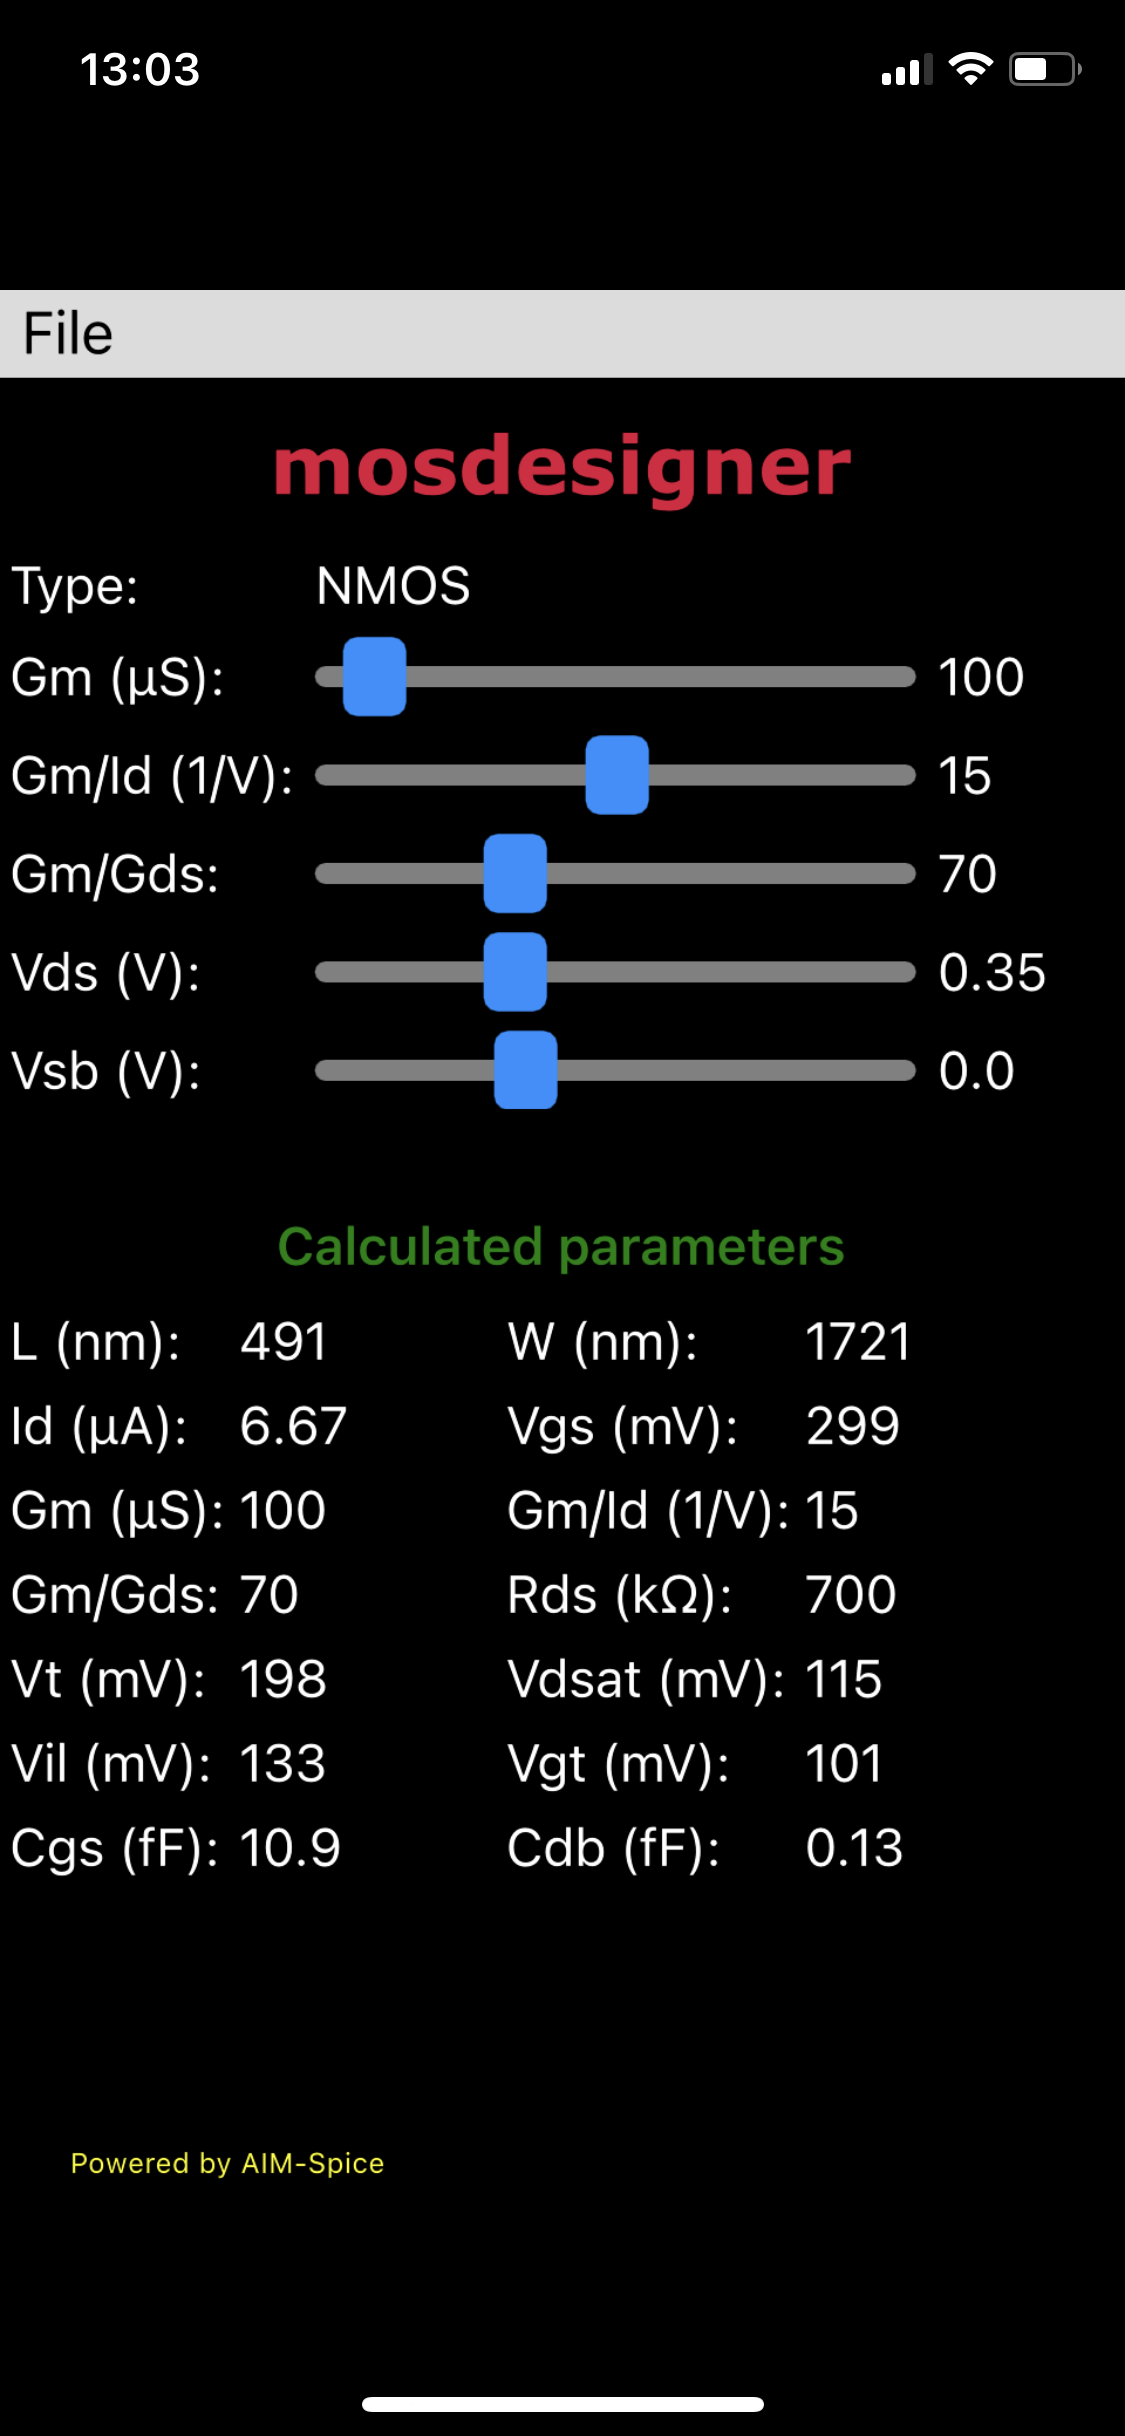
\includegraphics[height = 10cm, keepaspectratio]{Images/mosdesigner/NMOS_parameters.PNG}
        \caption{NMOS parameters}
        \label{fig:NMOS:param}
    \end{subfigure}%
    \begin{subfigure}{.33\textwidth}
        \centering
        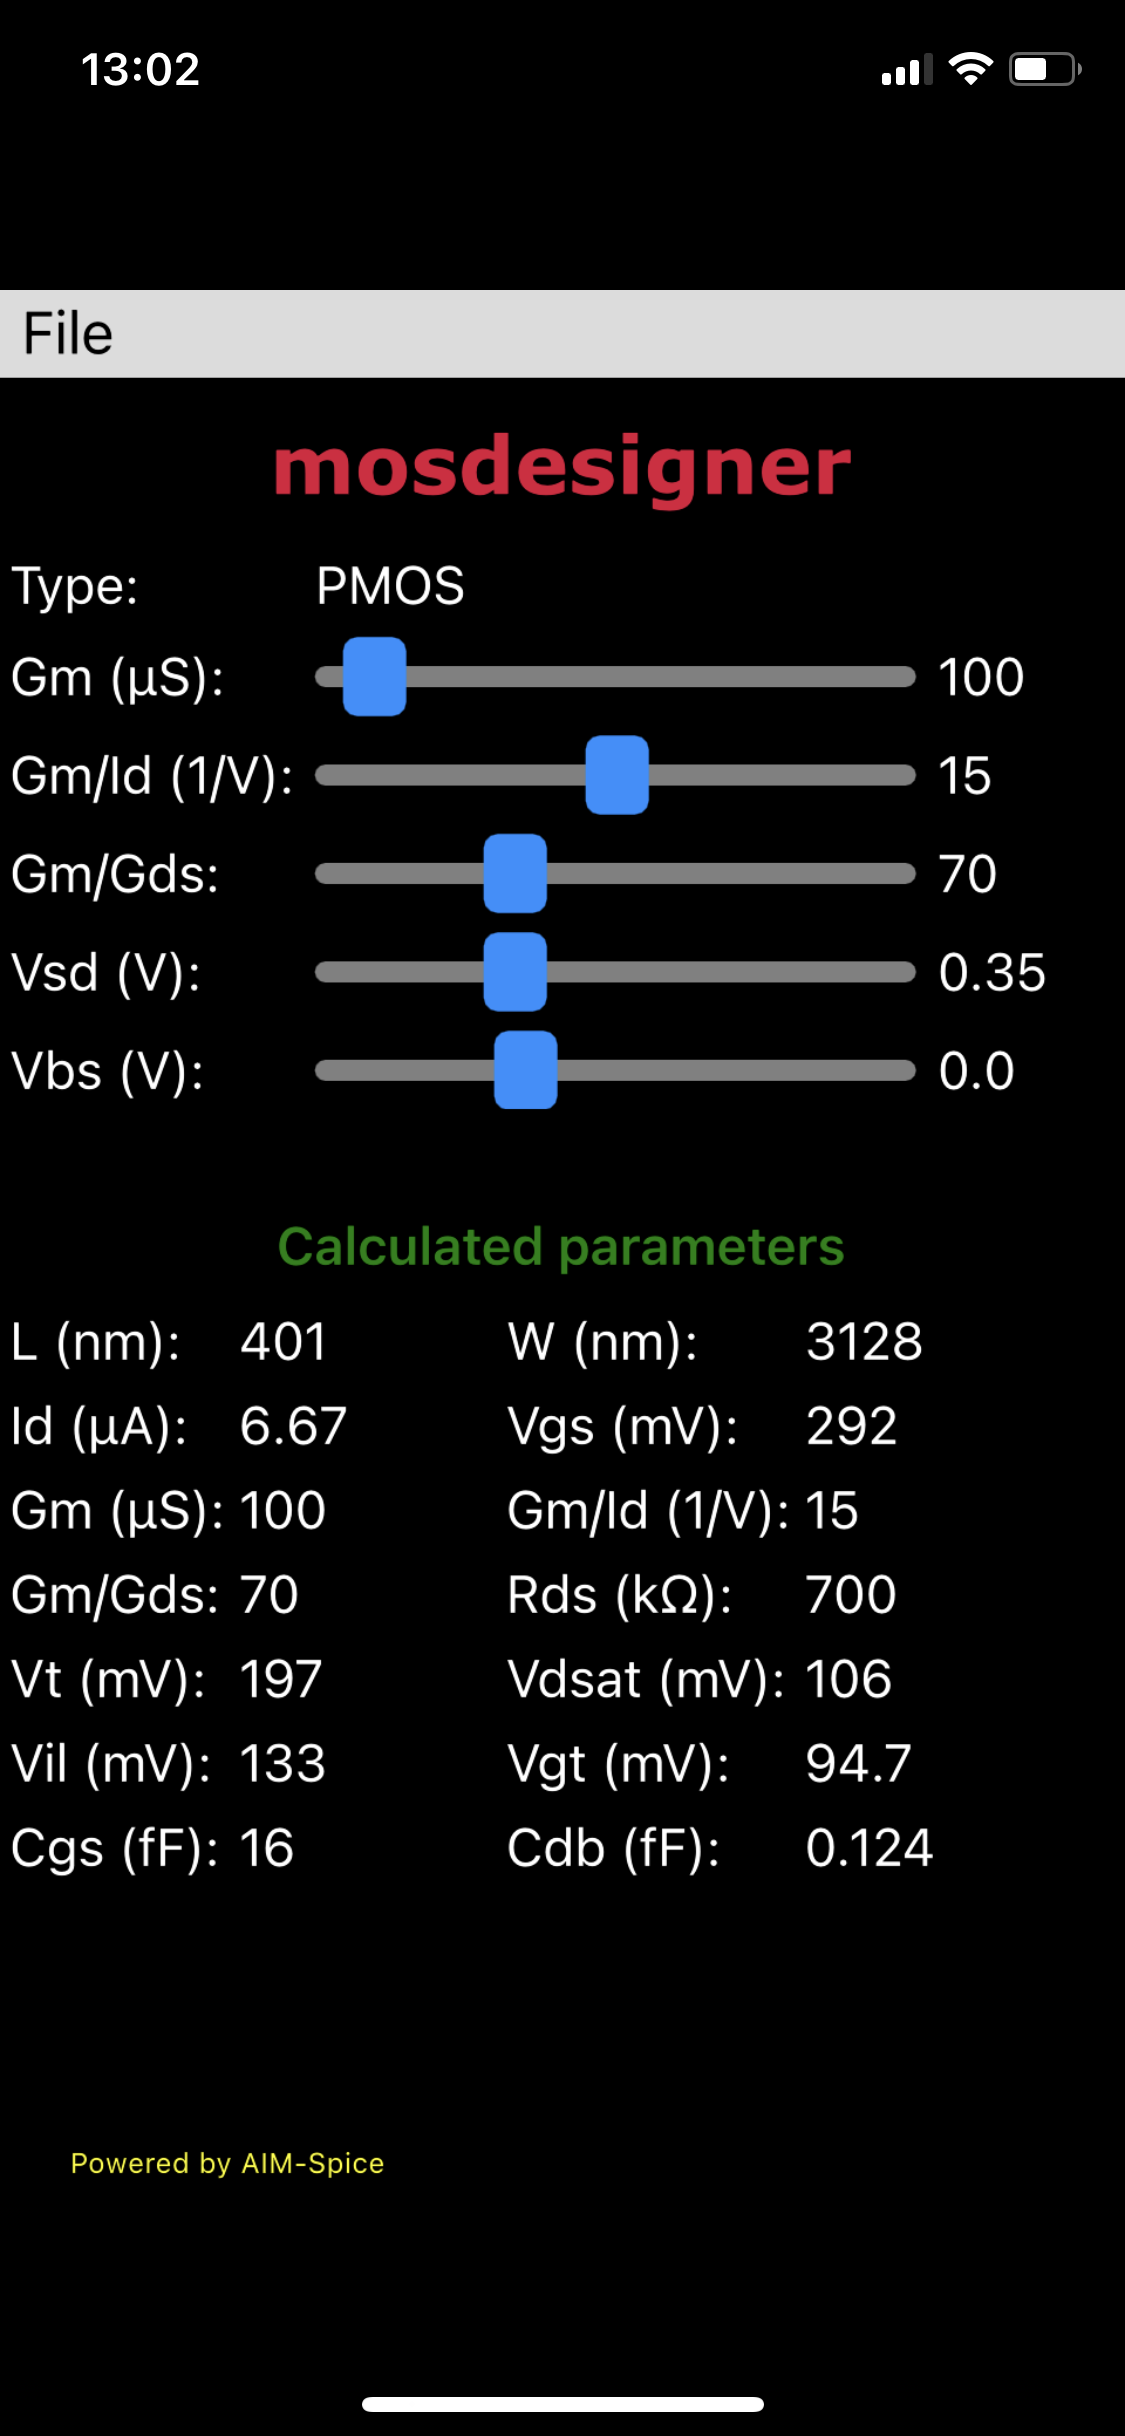
\includegraphics[height = 10cm, keepaspectratio]{Images/mosdesigner/PMOS_parameters.PNG}
        \caption{PMOS parameters}
        \label{fig:PMOS:param}
    \end{subfigure}%
    \begin{subfigure}{.33\textwidth}
        \centering
        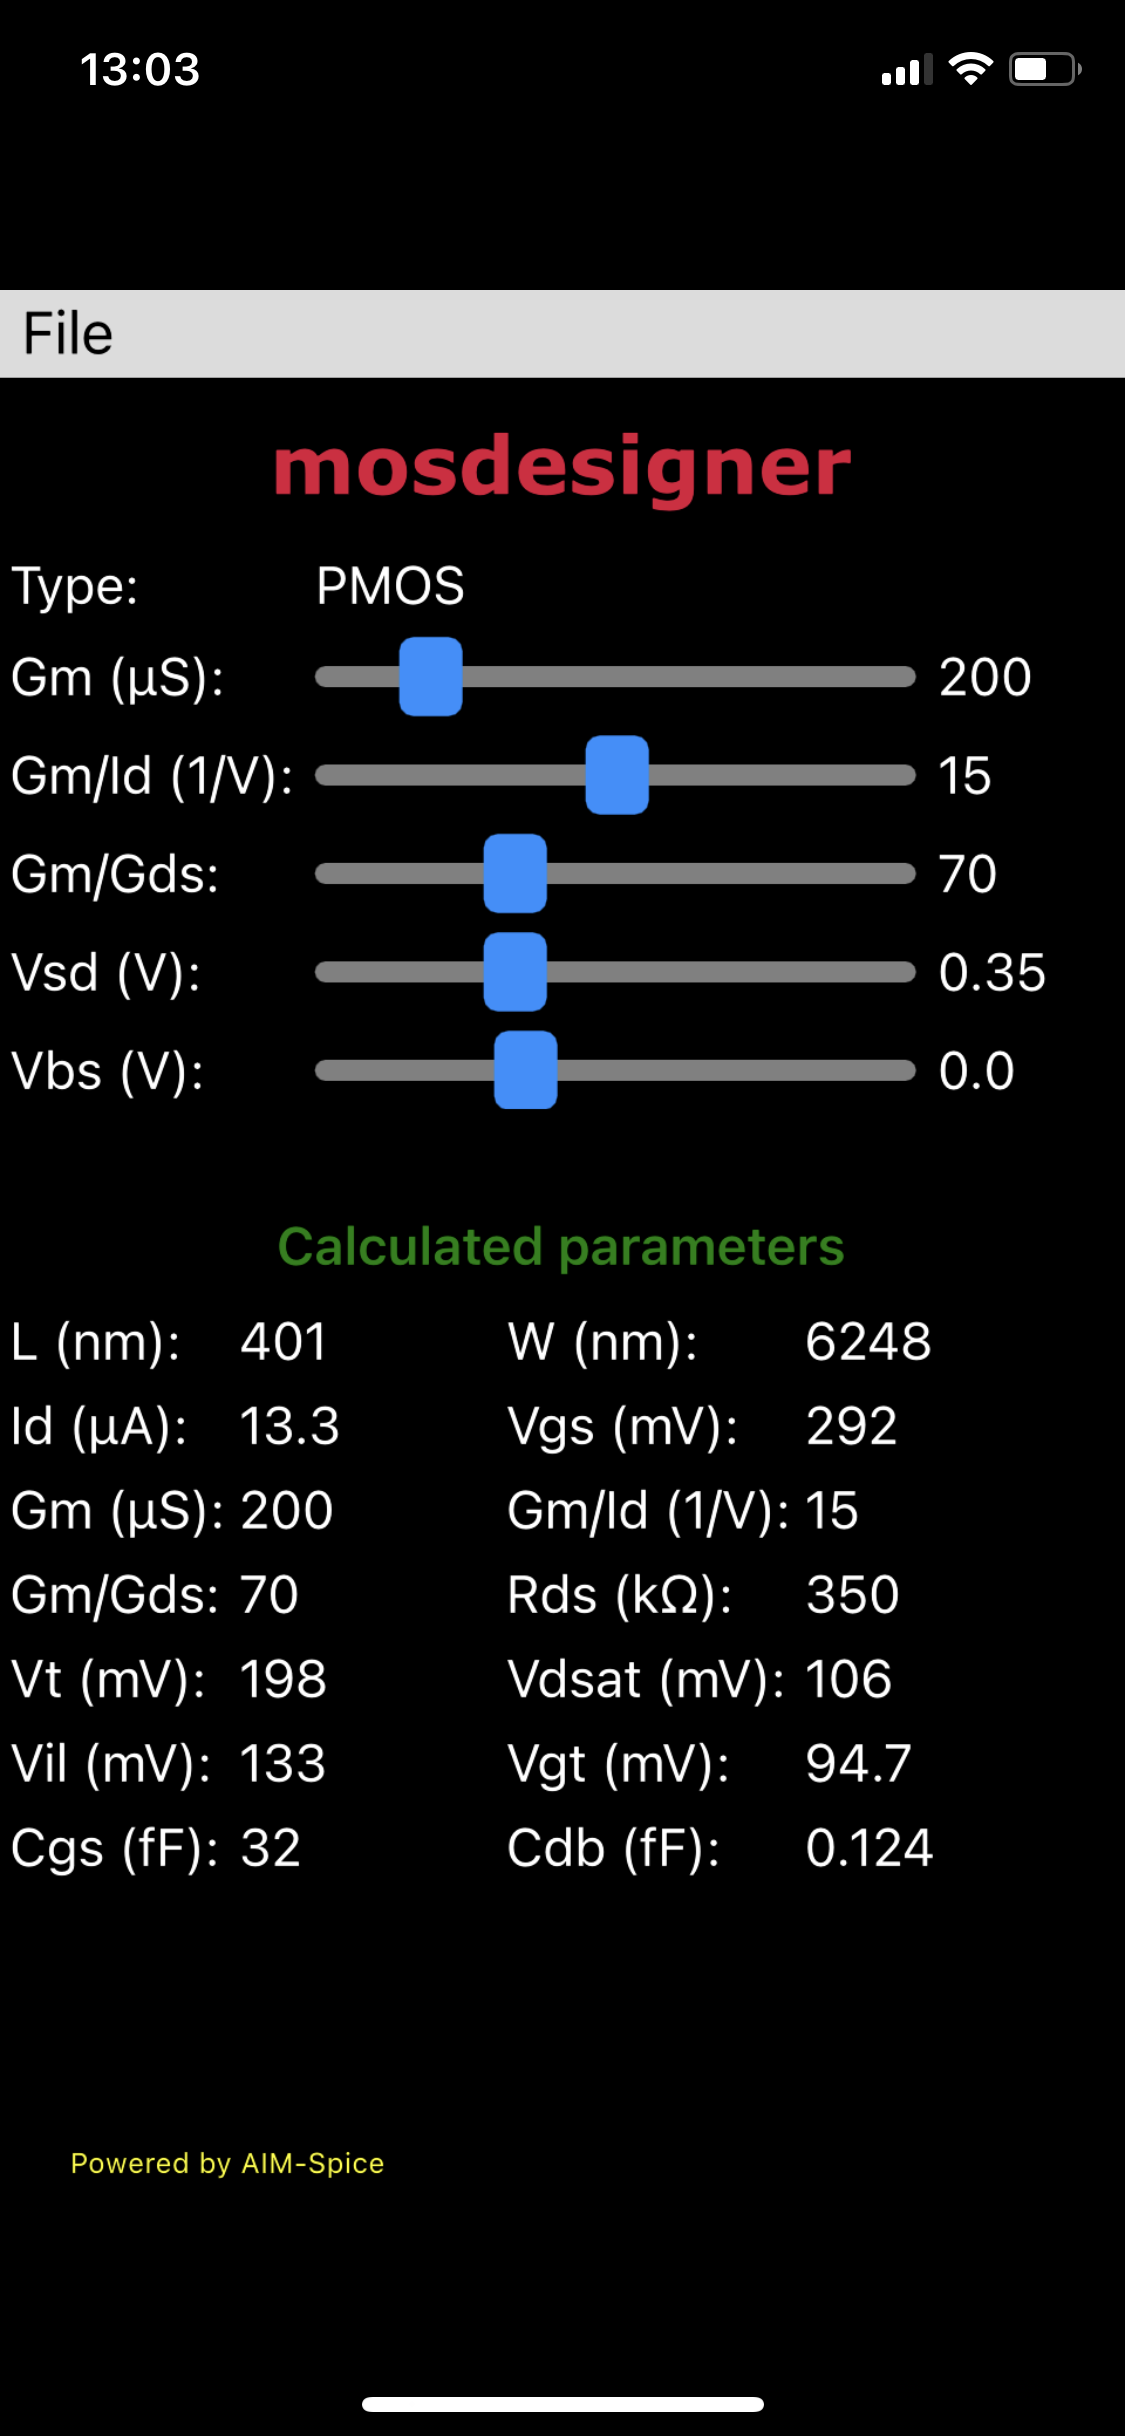
\includegraphics[height = 10cm, keepaspectratio]{Images/mosdesigner/PMOS_input_parameters.PNG}
        \caption{Bias PMOS parameters}
        \label{fig:PMOS:bias:param}
    \end{subfigure}
    \caption{Transistor parameters from \textit{mosdesigner} using the values from the hand calculations}
    \label{fig:transistor:param}
\end{figure}

As the PMOS input from the current mirror \textit{Q5} has to be able to bias the differential input gain stage \textit{Q1, Q2, Q3} and \textit{Q4}.  The current through \textit{Q5} needs to be twice the branch current of the differential stage to be able to bias both branches with the required current. Hence the bias PMOS transistor needs to be twice the width of the ones in the differential stage, as shown in figure \ref{fig:transistor:param}.

The circuit was setup in \textit{Cadence Virtuoso} as shown in figure \ref{fig:OTA:sch}
\begin{figure}[!htbp]
    \centering
    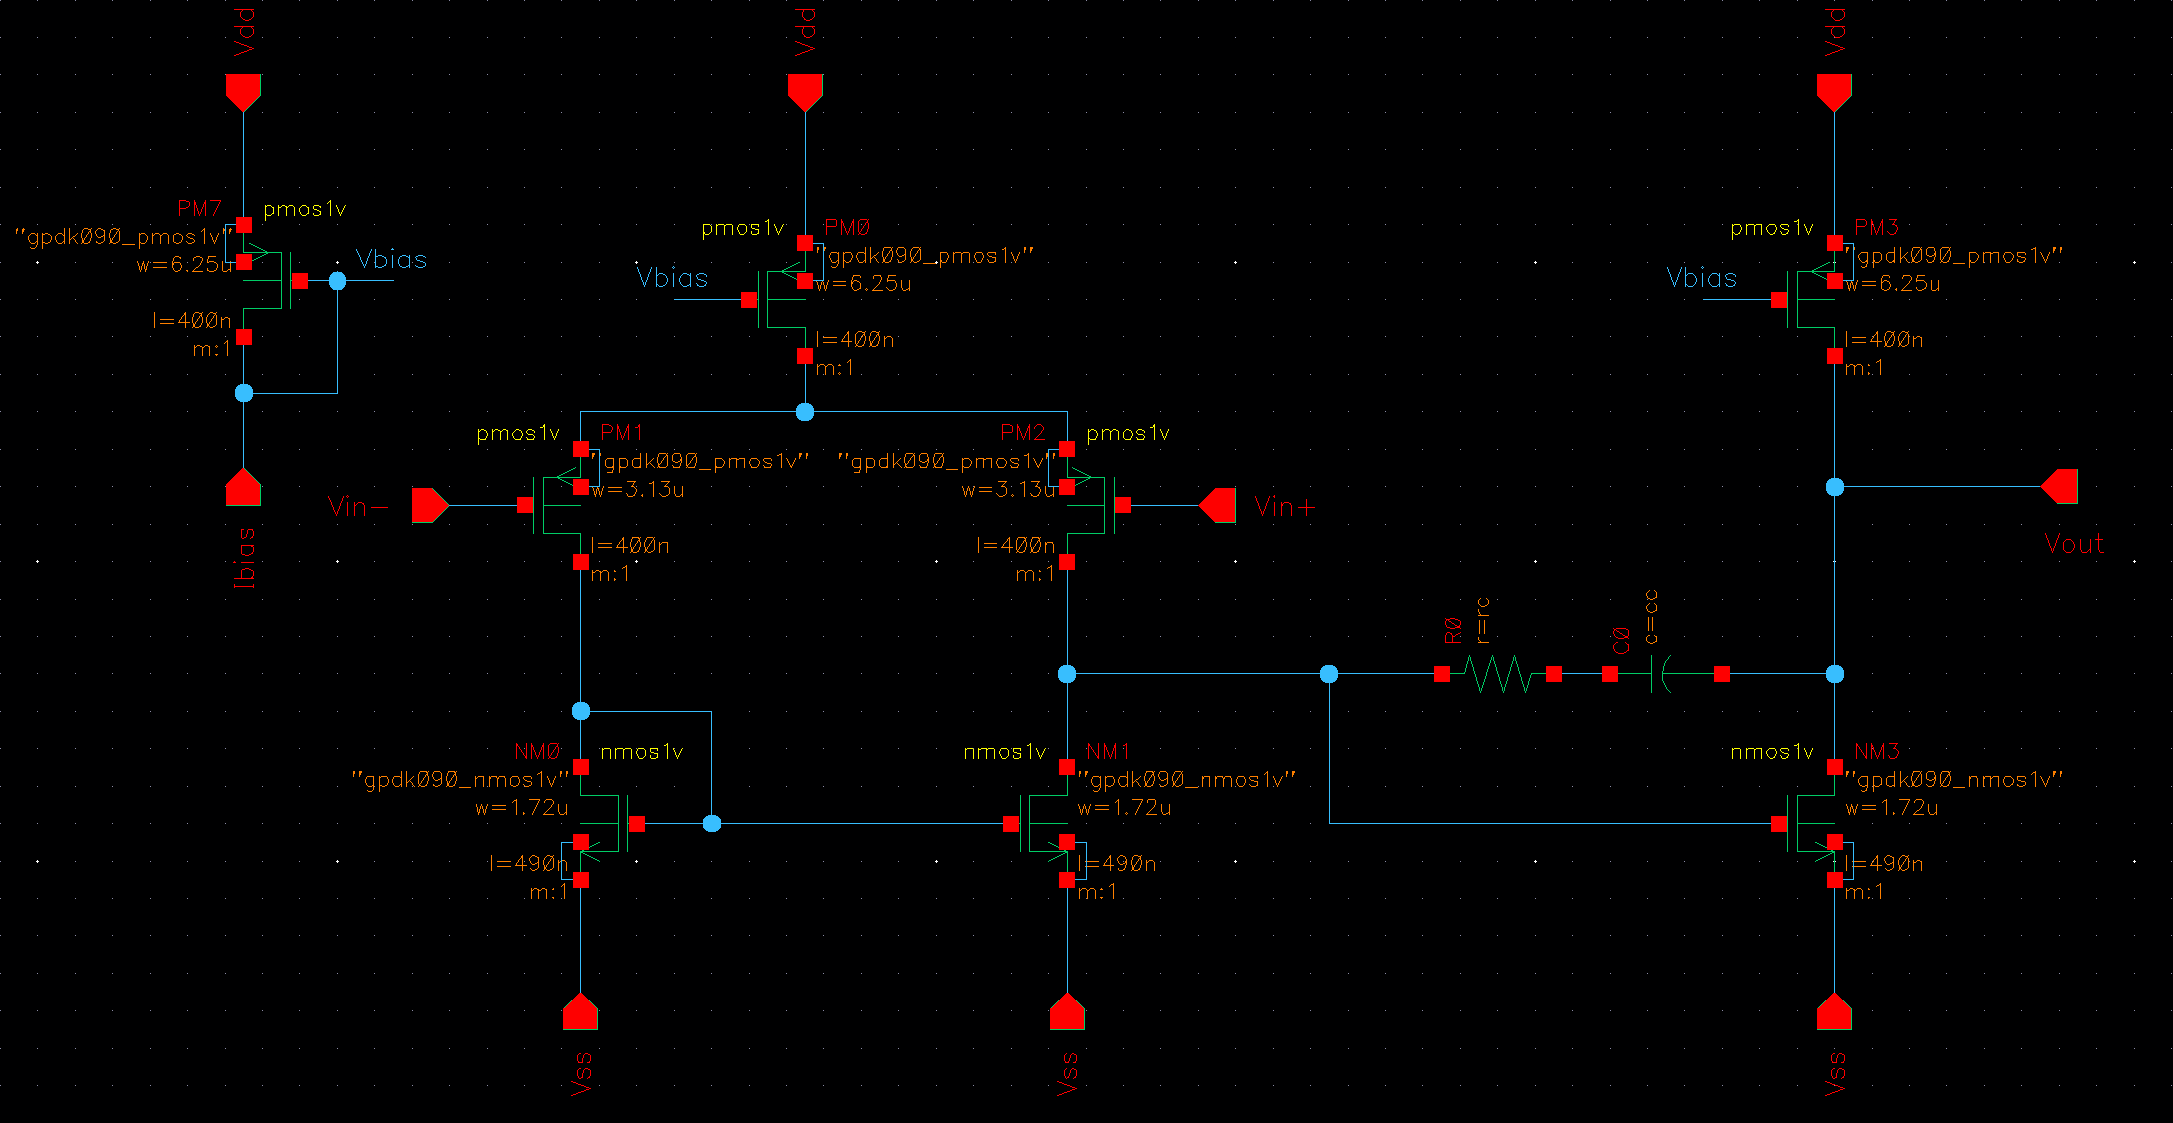
\includegraphics[width=.9\linewidth]{Images/Virtuoso/Miller_OTA_Virtuoso_sch.png}
    \caption{OTA setup in \textit{Virtuoso}}
    \label{fig:OTA:sch}
\end{figure}